\documentclass{beamer}
% \usefonttheme{professionalfonts}
\usefonttheme{professionalfonts}

\usepackage{amsmath}
\usepackage{cancel}
%%%%%%%%%%%%%%%%%%%%%%%%% For making hand-outs %%%%%%%%%%%%%%%%%%%%%%%%%%%
% \documentclass[handout]{beamer}
% \usepackage{pgfpages}
% \pgfpagesuselayout{2 on 1}[a4paper,border shrink=5mm]
%%%%%%%%%%%%%%%%%%%%%%%%%%%%%%%%%%%%%%%%%%%%%%%%%%%%%%%%%%%%%%%%%%%%%%%%%%
\definecolor{inputred}{HTML}{c30e0e}
\definecolor{hiddenblue}{HTML}{2626c9}
\definecolor{outputgreen}{HTML}{008000}
\newcommand{\figheight}{0.72\textheight}
% \usepackage{eulervm}
\usepackage{default}
\usepackage{caption}
\usepackage{booktabs,mathptmx,siunitx}
% \usefonttheme{serif}
\graphicspath{{img/}}
\captionsetup{font=scriptsize, labelfont=scriptsize}


\usepackage{showexpl}



\begin{document}



\begin{frame}[fragile]

\centering\Huge Block Practical: Connectionist models and cognitive processes
\vfill \huge
\centering Part 3: \textbf{Feedforward Networks} \large
\vfill
\textit{
Olivia Guest }

\end{frame}


\begin{frame}[fragile]
\frametitle{2-layer Perceptron}
\framesubtitle{Simplest form of network}
 \begin{columns}[T]
    \begin{column}{.45\textwidth} 
        \  \\
 \   \\ 
\begin{itemize}
\item Linearly separable datasets only

\ \\

 \item Cannot solve XOR-like problems
 
 \ \\
 
\item We need something more human-like in problem solving abilities! 
\end{itemize}
\end{column}
\begin{column}{.55\textwidth}
\begin{figure}[t]
 \begin{flushleft}

%  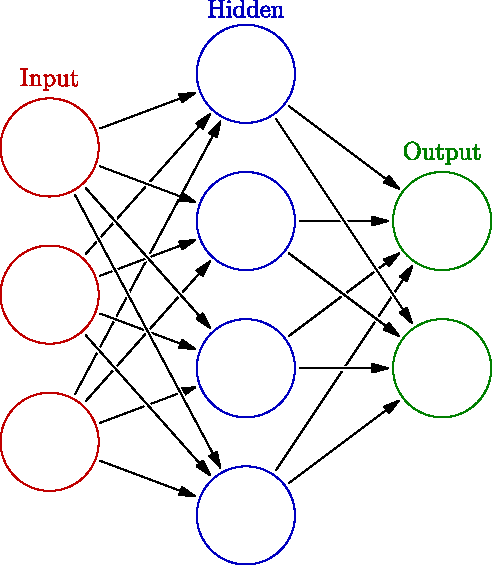
\includegraphics[height = \figheight]{./fig/3-layer.pdf}
  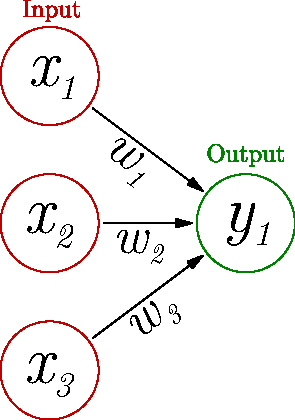
\includegraphics[height = \figheight]{./fig/perceptron_maths.pdf}

 \end{flushleft}
%  \caption{Glosser.ca / CC-BY-SA-3.0}
\end{figure}
\end{column}

\end{columns}

\end{frame}




\begin{frame}[fragile]
\frametitle{3-layer Perceptron}
\framesubtitle{Just add hidden units!}
 \begin{columns}[T]
    \begin{column}{.45\textwidth} 
             \  \\
 \   \\      
\begin{itemize}[<+->]

\item Can solve most problems

\ \\

 
\item As before we use targets to find the error for the output states... 
$\delta_i = y_i - t_i $

\ \\

 
 \item But how do we train the hidden units? 
\end{itemize}
\end{column}
\begin{column}{.55\textwidth}
\begin{figure}[t]
 \begin{flushleft}

 \includegraphics<1>[height = \figheight]{./fig/3-layer.pdf}
 \includegraphics<2->[height = \figheight]{./fig/3-layer_maths.pdf}


 \end{flushleft}
\end{figure}
\end{column}

\end{columns}
\end{frame}
\begin{frame}[fragile]
\frametitle{3-layer Perceptron}
\framesubtitle{Feedforward phase}
 \begin{columns}[T]
    \begin{column}{.45\textwidth} 
             \  \\
 \   \\   
     
     
\begin{itemize}
\item Run network as normal, i.e., feed activations forwards 

\ \\

 
\item When at output calculate error: 
$\delta_i = y_i - t_i $

\ \\

 
 \item But how do we calculate error for the hidden units?
\end{itemize}
\end{column}
\begin{column}{.55\textwidth}
\begin{figure}[t]
 \begin{flushleft}

 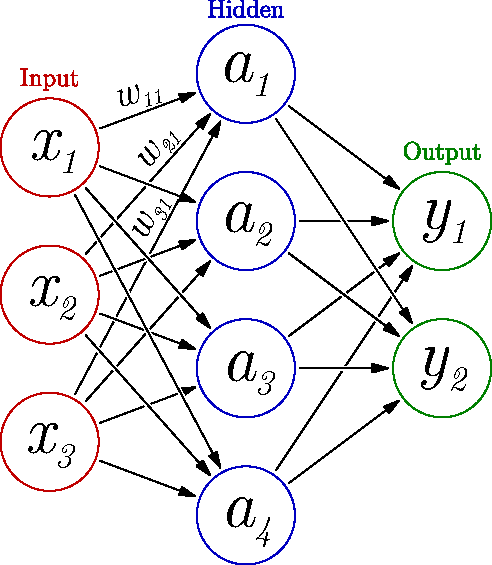
\includegraphics[height = \figheight]{./fig/3-layer_maths.pdf}


 \end{flushleft}
\end{figure}
\end{column}

\end{columns}
\end{frame}

\begin{frame}[fragile]
\frametitle{3-layer Perceptron}
\framesubtitle{Backpropagation phase}
 \begin{columns}[T]
    \begin{column}{.45\textwidth} 
             \  \\
 \   \\   
     
     
\begin{itemize}
\item Now the output is the starting point 

\ \\

 
\item When at output calculate error: 


\ \\

 
$\delta_i = y_i - t_i $


\ \\

 

 \item Now run the network backwards! 
\end{itemize}
\end{column}
\begin{column}{.55\textwidth}
\begin{figure}[t]
 \begin{flushleft}

 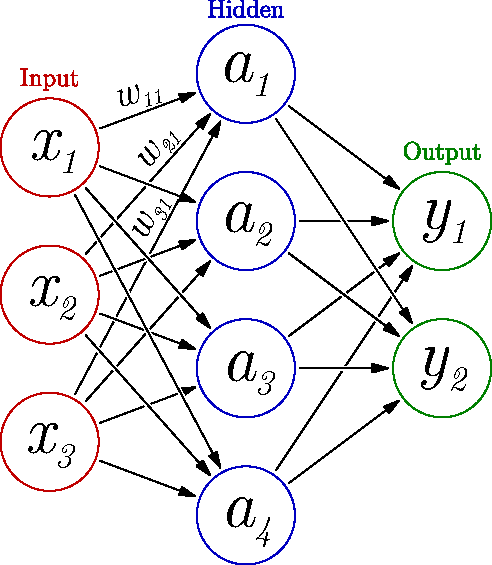
\includegraphics[height = \figheight]{./fig/3-layer_maths.pdf}


 \end{flushleft}
\end{figure}
\end{column}

\end{columns}
\end{frame}

\begin{frame}[fragile]
\frametitle{3-layer Perceptron}
\framesubtitle{Backpropagation phase}
 \begin{columns}[T]
    \begin{column}{.45\textwidth} 
             \  \\
 \   \\   
     
     
\begin{itemize}[<+->]
\item The hidden targets are: 
$  t_i = \sum_{j} \delta_j w_{ij} $


\ \\

 

 \item Now we  can calculate errors! 
 
 
\ \\

 
 Output error:
 
 
\ \\

 
$\delta_i = y_i - t_i $   
   
\ \\

 
   
   Hidden error:
   
   
\ \\

 
$\delta_i = a_i (1 - a_i)  t_i$
 
\end{itemize}
\end{column}
\begin{column}{.55\textwidth}
\begin{figure}[t]
 \begin{flushleft}

 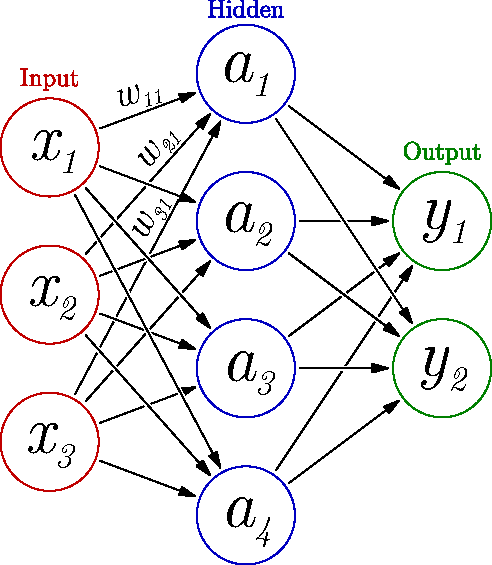
\includegraphics[height = \figheight]{./fig/3-layer_maths.pdf}


 \end{flushleft}
\end{figure}
\end{column}

\end{columns}
\end{frame}

\begin{frame}[fragile]
\frametitle{3-layer Perceptron}
\framesubtitle{Backpropagation phase}
 \begin{columns}[T]
    \begin{column}{.45\textwidth} 
             \  \\
 \   \\   
     
     
\begin{itemize}

\item<1-> Now we have our $\delta_i$s, we can calculate weight updates!
 \begin{center}

\ \\

 
\visible<2->{$\Delta w_{ij}= $} \visible<5->{$\sum_j$} \visible<3->{$\delta_j$} \visible<4->{$s_i$}
\end{center}



\ \\

 
 \item<6-> But --- before applying these updates --- we want to avoid local minima, so we have a few options...

 
\end{itemize}
\end{column}
\begin{column}{.55\textwidth}
\begin{figure}[t]
 \begin{flushleft}

 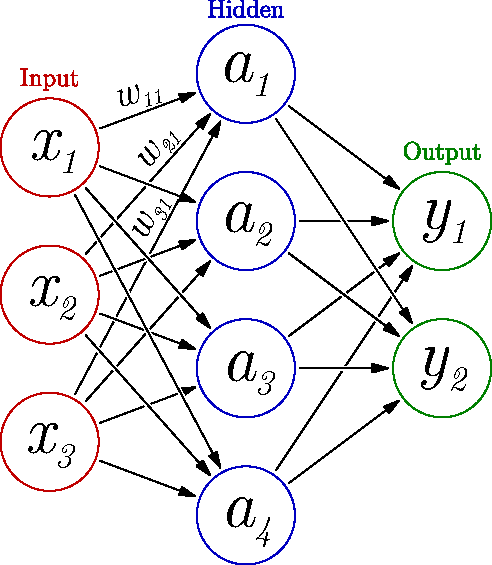
\includegraphics[height = \figheight]{./fig/3-layer_maths.pdf}

%   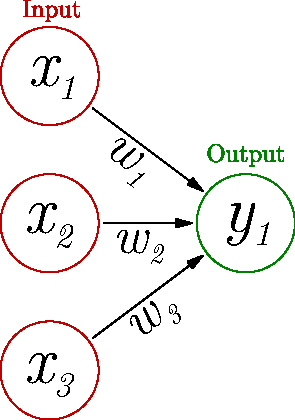
\includegraphics[height = \figheight]{./fig/perceptron_maths.pdf}

 \end{flushleft}
%  \caption{Glosser.ca / CC-BY-SA-3.0}
\end{figure}
\end{column}

\end{columns}
\end{frame}

\begin{frame}[fragile]
\frametitle{3-layer Perceptron}
\framesubtitle{Just before applying $\Delta w_{ij}$s consider...
}
\begin{itemize}[<+->]

\item Learning rate (too low too slow, too high too imprecise) 

\ \\

\item Initialisation of weights (random $\rightarrow$ different results) 

\ \\

\item Momentum:  move in a similar direction to last time; avoids noise affecting updates 

\ \\

\item Patternwise or in a batch? How to define a training epoch? 

\ \\

\item How to present patterns? In a random order? Serially?
\end{itemize}

\end{frame}

\begin{frame}[fragile]
\frametitle{3-layer Perceptron}
\framesubtitle{Applying weight changes!}
%  \begin{columns}[T]
%     \begin{column}{.45\textwidth} 

 

     
\begin{itemize}



 \item<1-> General equation for learning:
 
 \ \\
 
 \ \\
 \begin{center}
  


\visible<2->{$w_{ij}^{\epsilon +1} =$} \visible<3->{$w_{ij}^{\epsilon}$} \visible<5->{$ +  \nu \Delta w_{ij}^{\epsilon - 1}$} \visible<4->{$ - \mu \Delta w_{ij}^{\epsilon}$}
 \end{center}

  
 \ \\
 
 \ \\

 \visible<6-> {where $\epsilon$ denotes the epoch, the momentum is $\nu$, and the learning rate is $\mu$ --- latter two  can be either variable or constant. }
\end{itemize}

% \end{column}
% \begin{column}{.55\textwidth}
% \begin{figure}[t]
%  \begin{flushleft}
% 
%  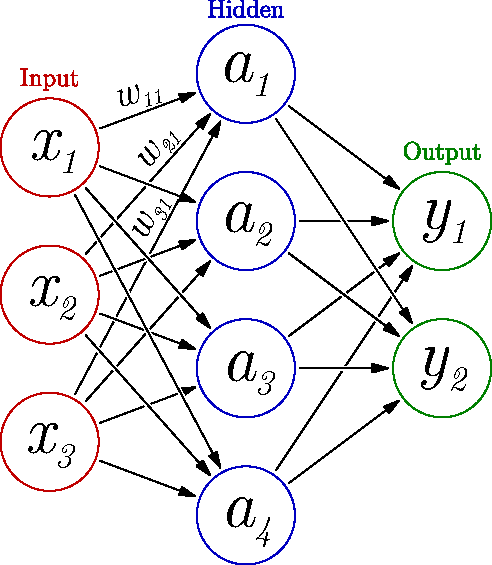
\includegraphics[height = \figheight]{./fig/3-layer_maths.pdf}
% 
% %   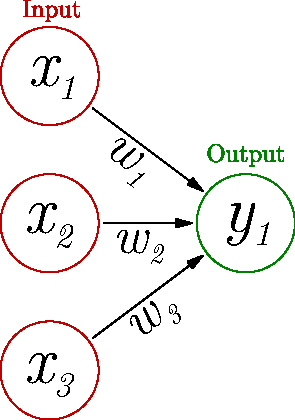
\includegraphics[height = \figheight]{./fig/perceptron_maths.pdf}
% 
%  \end{flushleft}
% %  \caption{Glosser.ca / CC-BY-SA-3.0}
% \end{figure}
% \end{column}
% 
% \end{columns}
\end{frame}




\begin{frame}[fragile]
\frametitle{Bias Units aka Thresholds}
\framesubtitle{What is it?}
 \begin{columns}[T]
    \begin{column}{.45\textwidth} 
             \  \\

     
\begin{itemize}[<+->]

\item A weight attached to a ``unit'' that is always on

\ \\

\item Trained identically to the weights


\ \\

\item Moves activation function left and right

 
\end{itemize}
\end{column}
\begin{column}{.55\textwidth}
\begin{figure}[t]
 \begin{flushleft}

 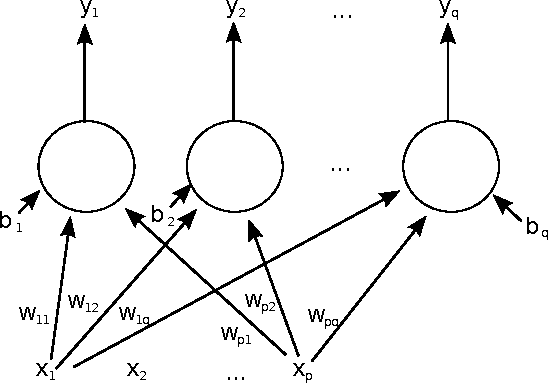
\includegraphics[scale=.65]{fig/Single_layer_ann.pdf}
%   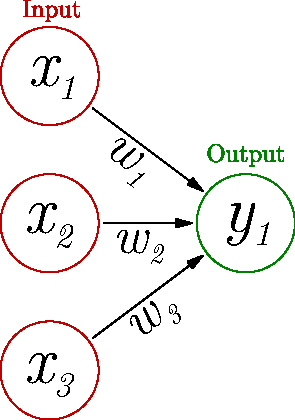
\includegraphics[height = \figheight]{./fig/perceptron_maths.pdf}

 \end{flushleft}
%  \caption{Glosser.ca / CC-BY-SA-3.0}
\end{figure}
\end{column}

\end{columns}
\end{frame}

\begin{frame}[fragile]
\frametitle{Activation Function}
\framesubtitle{Logistic, squashing, sigmoid, activation, step, etc., functions}
 \begin{columns}[T]
    \begin{column}{.45\textwidth} 
             \  \\

     
\begin{itemize}[<+->]

\item Generic  names: $f$, activation function, etc.

\ \\

\item Specific names: logistic function, hyperbolic tangent function, etc.


\ \\

\item Takes pre-synaptic input to a unit:
$ \eta_{i}= \sum_{j} s_jw_{ji} + b_i $



 
\end{itemize}
\end{column}
\begin{column}{.55\textwidth}
\begin{figure}[t]
 \begin{flushleft}

 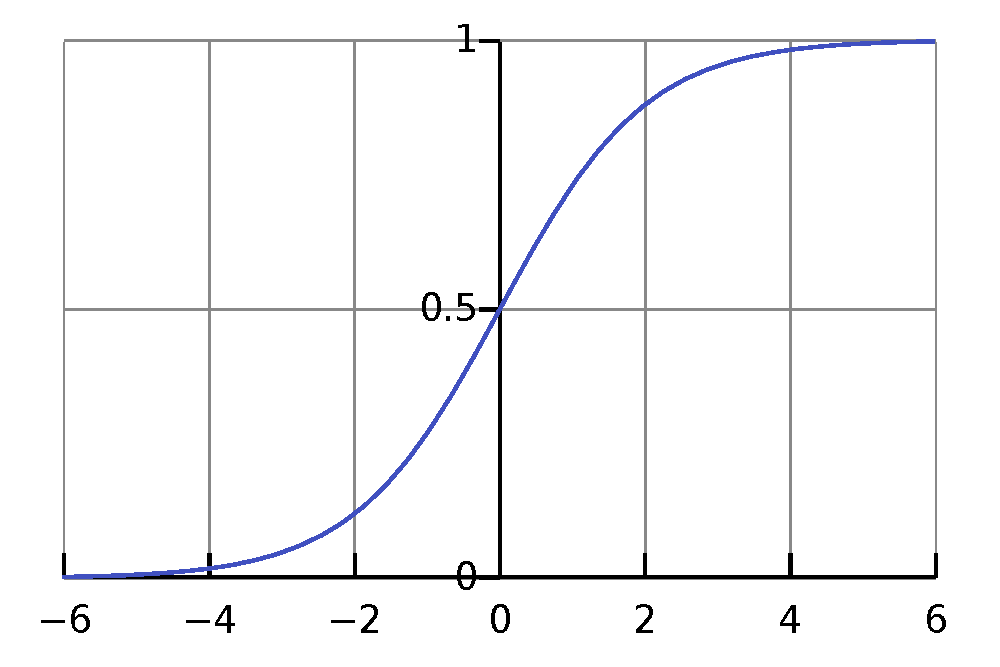
\includegraphics[scale=.4]{fig/Logistic-curve.pdf}
%   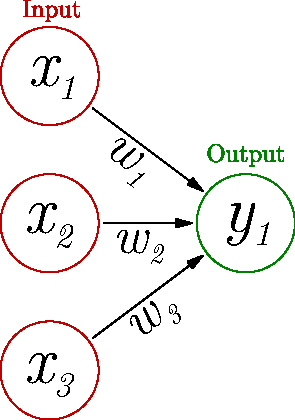
\includegraphics[height = \figheight]{./fig/perceptron_maths.pdf}


 \end{flushleft}
%  \caption{Glosser.ca / CC-BY-SA-3.0}
\end{figure}
\end{column}

\end{columns}
\end{frame}

\end{document}
